% !TeX program = xelatex
\documentclass[11pt,a4paper]{article}
\usepackage[margin=23mm]{geometry}
\usepackage{amsmath,amssymb,booktabs,array,tikz}
\usetikzlibrary{arrows.meta,positioning}
\usepackage[hidelinks]{hyperref}
\title{Path Planning for Multiple Mobile Robots:\\A Focused Review and an RMFS Experiment Design}
\author{Internal research note}
\date{November 21, 2026}
\begin{document}\maketitle
\noindent\textbf{Scope.} Route generation for multiple mobile robots, especially
warehouse fleets with finite bodies, turns, nonzero acceleration/braking, and
repeated tasks. Fixed-path traffic execution is a separate layer. This is a
targeted review, not a ranking of every planner or a claim of new methodology.
No planner architecture or controller code is changed by this work.

\section{First distinguish two multi-robot planning problems}
\begin{enumerate}
\item \textbf{Incremental fleet planning.} A robot receives a destination while
other robots already have routes and partially executed commands. Choose its
new route while retaining the other routes, subject to the existing traffic
controller. Waiting may change for every affected robot. This is not an isolated
single-robot problem, even if only one spatial route is variable.
\item \textbf{Joint fleet planning.} Given all starts and destinations, choose
the routes and schedules of several robots together. CBS-family and joint MAPF
methods can change several spatial routes to resolve a conflict. They have
more freedom than the incremental problem above.
\end{enumerate}
Using a joint replanner as a baseline for an incremental method without stating
that difference would be misleading. A roadmap $G=(V,E)$ need not be a regular
workspace grid. Conversely, using a roadmap does not by itself account for
collisions between finite robot bodies crossing geometrically adjacent edges.

\begin{center}
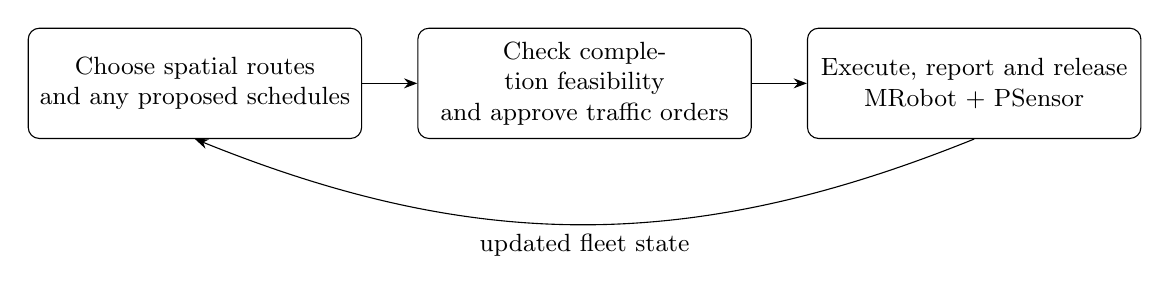
\begin{tikzpicture}[>=Stealth,box/.style={draw,rounded corners,align=center,text width=40mm,minimum height=14mm,font=\small}]
\node[box] (p) {Choose spatial routes\\and any proposed schedules};
\node[box,right=7mm of p] (c) {Check completion feasibility\\and approve traffic orders};
\node[box,right=7mm of c] (r) {Execute, report and release\\MRobot + PSensor};
\draw[->] (p)--(c);\draw[->] (c)--(r);
\draw[->] (r.south) to[bend left=22] node[below,font=\small] {updated fleet state} (p.south);
\end{tikzpicture}
\end{center}

\subsection*{The objective must be named}
For a finite one-shot batch, arrival times $C_i$ give
\begin{equation}
C_{\max}=\max_i C_i,\qquad \bar C={1\over N}\sum_i C_i.
\end{equation}
Minimizing sum of arrival times is equivalent to minimizing their mean for the
same fixed set of $N$ robots; it is not makespan minimization. For lifelong
tasks, throughput, task delay and starvation require additional measures.
Shortest path length and shortest unimpeded travel time are useful baselines,
not interchangeable versions of these fleet objectives.

\clearpage
\section{Multi-robot method families and what to take from them}
\subsection*{CBS/CCBS: joint conflict resolution by replanning}
CBS searches a conflict tree, with constrained route searches underneath.
CCBS [1] brings real-valued action times and geometric collision predicates
to this structure. The inspected 2019 model uses translating non-rotating
finite agents, constant speed and instantaneous starts/stops, on a roadmap.
Its objective is sum of costs, not makespan. The experimental agents are discs.
The paper claims broader applicability of the framework, but implementing a
new shape/dynamics predicate is not the same as validating those claims for
our rectangular rack model. Later correctness qualifications appear below.

\subsection*{Prioritized planning with safe intervals: sequential route creation}
Earlier robots' planned trajectories become reservations for later robots.
SIPP compresses waiting opportunities into safe intervals; it is a low-level
route-search building block, not by itself a complete multi-robot planner.
PSIPP/CTC [2] targets continuous-time planning on 2D roadmaps and precomputes
vertex/edge conflict annotations. Its authors' project describes prioritized
planning as incomplete and shows wheeled-robot simulation including motion
timing effects. This review could inspect the project and publication metadata,
\emph{not the full article}; detailed dynamics and theorem claims are therefore
not inferred from the demonstrations. It is a promising practical baseline,
not a proven complete solver for our model.

\subsection*{TP-SIPPwRT: repeated pickup-and-delivery tasks}
TP-SIPPwRT [3] combines token-based task/route coordination with a reservation
table and SIPP route search. Its stated model has grid locations, disc bodies,
orientation, forward motion and point turns at specified speeds, but infinite
acceleration/deceleration. Its completion theorem requires well-formed MAPD:
finitely many tasks, sufficient non-task endpoints for the agents, and paths
between endpoints avoiding other endpoints. These are substantive layout/task
conditions, relevant to our earlier home-position discussions. The theorem is
not a completion guarantee for arbitrary rack/workstation arrangements.

\subsection*{RHCR: scalable lifelong replanning}
RHCR [4] plans within a conflict horizon $w$ and executes/replans with period
$h\le w$. It is evaluated using several windowed MAPF solvers, with flowtime
as the window objective and throughput in lifelong operation. Sections 4.3--4.4
explicitly demonstrate a too-short-horizon deadlock and discuss starvation even
with the proposed remedy. The paper does not claim completeness or optimality
of lifelong RHCR. Large simulated grid-agent counts must not be treated as
evidence for our acceleration-aware rectangular bodies without adaptation.

\subsection*{LaCAM* and SCALE: useful additional context}
LaCAM* provides scalable graph MAPF search; SCALE integrates planning with
geometric conflict checking and execution-order optimization. Both were reviewed
in the previous literature notes. Their graph-search successes do not make
them drop-in implementations of our Plant dynamics or event-based safety policy.
SCALE's MILP is not the whole route-generation algorithm.

\clearpage
\section{Motion realism and current continuous-time qualifications}
\subsection*{MAPF-POST: timing a route after it has been chosen}
MAPF-POST [5] postprocesses a MAPF solution with a simple temporal network,
including translation/rotation velocity bounds and safety distances. The paper
explicitly uses a uniform-velocity model requiring instantaneous velocity
changes at some events (PDF p.~5). It is not a direct acceleration-limited
global route optimizer. Its controller approximates the planned timing.
This distinction matters: changing the route objective can be necessary when
rotation and acceleration make distance-optimal routes slow.

\subsection*{SIPP-IP: a building block, not a joint fleet theorem}
SIPP-IP [6] includes velocity in configurations and preserves intervals of
reachable times rather than only the earliest arrival. It shows why ordinary
SIPP can fail when waiting is unavailable at a nonzero-velocity state. Its
completeness/optimality statements concern a single robot against known moving
obstacles, with specified motion primitives and integer time durations.
Putting it inside prioritized multi-robot planning does not automatically
provide multi-robot completeness, and it does not imply continuous-event Plant
execution must use fixed time steps.

\subsection*{Continuous time is not a settled blanket guarantee}
The latest inspected version of \emph{Revisiting CCBS} [7] is v4, November 18,
2026. It challenges CCBS correctness/termination with arbitrary real-valued
waiting and distinguishes that model from fixed-duration wait actions.
One should not repeat the original CCBS completeness claim unqualified.
These are the authors' results in their stated models; this review does not
independently verify every proof or settle the ensuing literature.

OC-CBS [8], v3 August 2026, develops repaired branching and claims exactness
and solution completeness under its stated finite-precision model. Section
3.2.1 explicitly excludes sufficiently tiny unresolved collision intervals.
That numerical policy must not be silently imported as physical permission
for robots to overlap; engineering margins and conservative collision
validation remain a separate requirement.

CBS-AA [9] addresses a different asynchronous-action abstraction: while
traversing an edge a robot occupies \emph{both endpoint vertices}. It minimizes
sum of arrival costs. The inspected PDF's Theorem 1 states optimality and
solution completeness, not necessarily finite failure detection on unsolvable
inputs. This duration-occupancy model does not detect arbitrary crossing-edge
or rack-body geometry without an appropriate encoding. Its statements therefore
cannot be used as an unrestricted geometric-continuous-time guarantee.

\paragraph{Practical lesson.}
Reserve ``optimal'' and ``complete'' for a named objective, state/action model,
collision predicate, numerical policy and termination condition. Availability
of an open-source solver is helpful but is not a substitute for this match.

\clearpage
\section{Our current MRobot changes how a time graph must be built}
The existing \texttt{motion.py} implements analytical rest-to-rest straight
profiles. Loaded values are $a=b=0.37$ m/s$^2$, $v=2$ m/s, and yaw rate
$30$ degrees/s. Empty values are $a=b=0.41$ and yaw rate $45$ degrees/s.
These are existing model parameters; the file explicitly calls braking and yaw
rates assumptions. They are not a newly verified MiR600 specification.

For straight distance $D>0$, define
\begin{align}
v_p(D)&=\min\!\left(v,\sqrt{\frac{2D}{1/a+1/b}}\right),\\
T(D)&=\frac{D}{v_p(D)}+\frac{v_p(D)}{2}\left(\frac1a+\frac1b\right).
\end{align}
Here $a,b>0$ are acceleration and braking magnitudes, $v$ is cruise speed,
and $v_p$ is the peak speed. The two cases are triangular and trapezoidal
profiles. The model's constant-yaw turn cost is $|\Delta\theta|/\omega$ with
angle and yaw rate expressed in matching units.

\textbf{Why an edge-only duration can be wrong.} Consecutive straight motion
does not restart from rest at every intermediate roadmap vertex. In general,
\begin{equation}
T(D_1+D_2)\ne T(D_1)+T(D_2).
\end{equation}
Summing independent rest-to-rest durations over elementary grid edges inserts
stops that the Plant does not make. Conversely, removing every intermediate
stop is wrong when a traffic command requires one. Motion time must reflect
the actual command grouping, heading and stopping assumptions.

\begin{center}
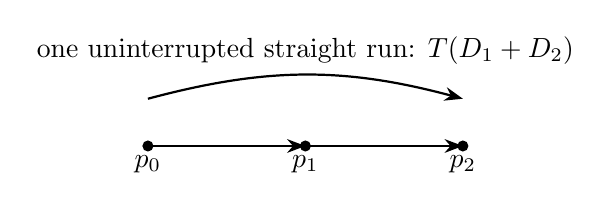
\begin{tikzpicture}[>=Stealth]
\foreach \x/\name in {0/$p_0$,2/$p_1$,4/$p_2$} {
\fill (\x,0) circle(2pt);\node[below] at (\x,0) {\name};}
\draw[->,thick] (0,0)--(2,0);\draw[->,thick] (2,0)--(4,0);
\draw[->,thick] (0,.6) to[bend left=15] node[above] {one uninterrupted straight run: $T(D_1+D_2)$} (4,.6);
\end{tikzpicture}
\end{center}

\paragraph{Suitable first baseline design, not yet an implementation.}
For static unimpeded travel, use heading-aware states and straight-run macro
edges with rest-to-rest boundary conditions, charging turns at direction
changes. Intermediate vertices may be passed. If arbitrary nonzero-velocity
state transitions are required, include velocity/motion primitives instead.
Adding velocity is not an optional cosmetic detail when dynamic constraints
make an earlier arrival unable to wait. For dynamic traffic, a new forced stop
can change subsequent durations; it must be replanned or reevaluated.

\clearpage
\section{A bounded, fair first study for our fleet}
\subsection*{Stage A: isolate the route-time issue}
Use the same starts, goals, footprints, initial headings and motion limits for
all methods. Compare shortest-distance routing with heading/motion-time routing
on small roadmaps, including equal-distance zigzag and L-shaped routes. This
is a calibration experiment, not the multi-robot result. Check predicted travel
times against the existing MRobot model before adding traffic.

\subsection*{Stage B: incremental multi-robot routing}
Keep the other robots' spatial routes fixed and use the same FIFO traffic
controller and completion checks for every candidate. Compare:
\begin{enumerate}
\item shortest-distance route with a stated deterministic tie rule;
\item shortest unimpeded motion-time route under the validated motion model;
\item several feasible route candidates evaluated from the same DEVS snapshot
to finite-batch completion, choosing the best observed fleet objective.
\end{enumerate}
The third method is a heuristic over its candidate set, not a global optimum.
Failure of our selected completion test must not be mislabeled as physical
infeasibility. Future dynamic routes should not disappear from a lookahead
branch merely because they have not yet been planned in that branch.

\subsection*{Stage C: an external baseline with matched freedom}
A prioritized continuous-time reservation planner is the most natural first
external \emph{incremental} comparison. PSIPP/CTC is a candidate; full-paper
and implementation inspection is still needed. Explicitly match body geometry,
turn/stopping rules, other robots' commitment rights, goal persistence and
safety margins. If the baseline uses deterministic reservations while our
controller admits uncertain event timing, report that assumption difference.
Small joint-planning comparisons can use a CBS-family reference separately;
do not call a disc/constant-speed result a rectangle/acceleration baseline.

\subsection*{Cases and measurements}
Start with 2, 3, 5 and 10 robots: a direct crossing, a same-direction merge,
opposing narrow traffic with a bypass, several coupled intersections, and a
warehouse rack-to-workstation case. Fix random seeds and retain the instances.
Report $C_{\max}$, mean and standard deviation of $C_i$, planning runtime,
candidate count, feasible/failed/timeout outcomes, path length, turn count,
traffic wait and changed-stop count. Add success rate across repeated instances.
Do not infer scalability from one best-case scene or count animation time as
planner time.

Search and snapshot rollouts should remain headless/event-driven, with no
animation sampling or periodic release polling. Geometry needed for planning
feasibility is still required. For final replay validation, enable the separate
collision checker with \emph{stop on collision}, and state its sampling interval
and limitations. Sampled replay is not a continuous collision-freedom proof.
No new architecture is authorized by this proposed experiment design.

\clearpage
\section{Conclusions and reading record}
\begin{enumerate}
\item Multi-mobile-robot path planning already includes route changes, continuous
time, finite bodies, turns, reservations, repeated tasks and dynamics-aware
subproblems. None of these features alone should be presented as new.
\item No inspected method is automatically a drop-in match for our complete
rectangular-envelope, acceleration-aware, event-controlled RMFS. Matching
assumptions is required, but that difference does not by itself prove novelty.
\item The first useful study is whether motion-time route choice and then fleet
interference change which path performs best. A snapshot evaluator is an
experimental tool for that question, not a claim that prior work lacks foresight.
\end{enumerate}

Eight full PDFs were downloaded locally. Reading focused on problem statements,
state/action definitions, algorithms and guarantee assumptions. Sections read
include CCBS Secs.~2--4; the token policy, model and Theorems 1--2 of TP-SIPPwRT; RHCR
Secs.~3--4.4; MAPF-POST uniform-velocity and non-holonomic sections; SIPP-IP
formulation, counterexample and theorem sections; and the recent CCBS papers'
formulations, branching/guarantee and numerical-assumption sections. This is not
a claim that every proof on every page has been independently verified.

PSIPP/CTC was inspected through the authors' project page and publication
metadata only. The 2015 CBS journal PDF download failed and is not counted as
a read primary paper here. Existing SCALE/LaCAM* notes supply background, not
new reproductions. No external solver was built or benchmarked. The existing
research manuscript, Korean documents, TrafficManager and RobotPathPlanner
implementation are unchanged.

\begin{thebibliography}{9}\small
\bibitem{ccbs} A. Andreychuk et al., ``Multi-Agent Pathfinding with Continuous
Time,'' IJCAI, 2019. \url{https://ijcai.org/proceedings/2019/0006.pdf}.
\bibitem{psipp} K. Kasaura, M. Nishimura, R. Yonetani, ``Prioritized Safe
Interval Path Planning for Multi-Agent Pathfinding With Continuous Time on 2D
Roadmaps,'' RA-L, 7(4), 10494--10501, 2022. Authors' project:
\url{https://omron-sinicx.github.io/PSIPP-CTC/}.
\bibitem{tp} H. Ma et al., ``Lifelong Path Planning with Kinematic Constraints
for Multi-Agent Pickup and Delivery,'' AAAI, 2019. Inspected preprint:
\url{https://arxiv.org/abs/1812.06355}.
\bibitem{rhcr} J. Li et al., ``Lifelong Multi-Agent Path Finding in Large-Scale
Warehouses,'' AAAI, 2021. \url{https://jiaoyangli.me/files/2021-AAAI-2.pdf}.
\bibitem{post} W. H\"onig et al., ``Multi-Agent Path Finding with Kinematic
Constraints,'' ICAPS, 2016. \url{https://whoenig.github.io/publications/2016_ICAPS_Hoenig.pdf}.
\bibitem{ip} Z. A. Ali, K. Yakovlev, ``Safe Interval Path Planning With
Kinodynamic Constraints,'' AAAI, 2023. \url{https://arxiv.org/abs/2302.00776}.
\bibitem{revisit} A. Li et al., ``Revisiting Conflict-Based Search with
Continuous-Time,'' arXiv:2501.07744v4, November 18, 2026.
\url{https://arxiv.org/abs/2501.07744v4}.
\bibitem{oc} A. Combrink, S. F. Roselli, M. Fabian, ``Optimal Multi-Agent Path
Finding in Continuous Time,'' arXiv:2508.16410v3, August 8, 2026.
\url{https://arxiv.org/abs/2508.16410v3}.
\bibitem{aa} X. Wu, S. Zhao, Z. Ren, ``Conflict-Based Search for Multi Agent
Path Finding with Asynchronous Actions,'' arXiv:2603.18866, 2026.
\url{https://arxiv.org/abs/2603.18866}.
\end{thebibliography}
\end{document}
